\section{Implementing iCareData}
\label{chap:iCareData}
From the System Designer's point of view, the project is divided into two parts. The building and its inhabitants. 
\\
The iCareData part is called periodically by the server. The tasks are to manage the data of the residents and to define the building. Figure \ref{fig:iCareDataBuilding} on the following page shows the basic structure of the building part. It consists of two interfaces and classes that represent each room in the building. 
\subsection{Object models}
Each room is a composition of a door as well as bounds. The bounds are important for the building because it contains the architectural measurement of each room. This will also get more important when the building and its inhabitants are displayed on the web page. The door is basically important for the frontend. The position of the doors will make sure, that the inhabitants will walk through them and not through the walls. The two interfaces consist of the coordinates of the entire building and will make sure that every class will implement the right methods.
\begin{figure}[h]
	\centering
	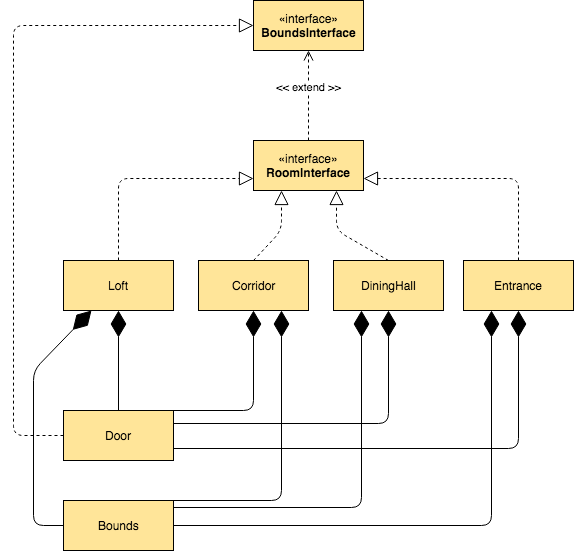
\includegraphics[width=\textwidth]{images/iCareDataBuilding}
	\caption{Object Diagram iCareData Building}
	\label{fig:iCareDataBuilding}
\end{figure}
\clearpage
Figure \ref{fig:iCareDataInhabitant} shows the second part of the iCareData project. It is dedicated to the inhabitants. Each resident is a composition of a healthCheck and a position.
\\
The aim of HealthCheck is to receive the sensor data and make it available to the server as processed data. The data is polled and handled by the CPU from chapter \ref{market-analysis}. For example, if the heart rate comes in a critical state, an alarm is triggered immediately. The data used for this purpose is stored in the resident's object so that it can be displayed on the website. In this way, employees are also visually informed that something is wrong.
\begin{figure}[h]
	\centering
	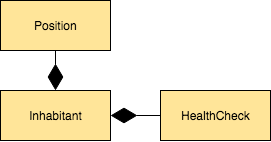
\includegraphics[width=.5\textwidth]{images/iCareDataInhabitant}
	\caption{Object Diagram iCareData Inhabitant}
	\label{fig:iCareDataInhabitant}
\end{figure}
The position is determined as a combination of motion detectors and smart wristbands. However, this is only the case when people need special treatment because they need to be under observation. It is therefore important to know where they are. The information in the healthCheck and the position can be used to determine exactly where a patient is in an emergency.
